\documentclass[10pt,twocolumn,letterpaper]{article}

\usepackage{cvpr}
\usepackage{times}
\usepackage{epsfig}
\usepackage{graphicx}
\usepackage{amsmath}
\usepackage{amssymb}
\usepackage[utf8]{inputenc}

% Include other packages here, before hyperref.

% If you comment hyperref and then uncomment it, you should delete
% egpaper.aux before re-running latex.  (Or just hit 'q' on the first latex
% run, let it finish, and you should be clear).
\usepackage[breaklinks=true,bookmarks=false]{hyperref}

\cvprfinalcopy % *** Uncomment this line for the final submission

\def\cvprPaperID{****} % *** Enter the CVPR Paper ID here
\def\httilde{\mbox{\tt\raisebox{-.5ex}{\symbol{126}}}}

% Pages are numbered in submission mode, and unnumbered in camera-ready
%\ifcvprfinal\pagestyle{empty}\fi
\setcounter{page}{1}
\begin{document}

%%%%%%%%% TITLE
\title{Evaluaci\'on de M\'etodos de Segmentación de Im\'agenes Usando la Base de Datos BSDS500}

\author{Francisco J. Cedano\\
Departamento de Ingenier\'ia Biom\'edica\\
Universidad de Los Andes\\
{\tt\small fj.cedano803@uniandes.edu.co}
% For a paper whose authors are all at the same institution,
% omit the following lines up until the closing ``}''.
% Additional authors and addresses can be added with ``\and'',
% just like the second author.
% To save space, use either the email address or home page, not both
}%\and
%Second Author\\
%Institution2\\
%First line of institution2 address\\
%{\tt\small secondauthor@i2.org}


\maketitle
%\thispagestyle{empty}

%%%%%%%%% ABSTRACT
\begin{abstract}
   Este informe estudia dos diferentes algoritmos para segmentaci\'on de im\'agenes usando la base de datos BSDS500 de Berkley para evaluaci\'on de estos algoritmos en 200 im\'agenes. El primer algoritmo es basado en kmeans y el segundo es basado en el modelo de mezclas gaussianas (gmm). Ambos algoritmos son evaluados a partir de curvas precisi\'on-cobertura. Se encontr\'o que mezclas gaussianas tiene un mejor rendimiento en esta evaluaci\'on respecto a kmeans.
\end{abstract}

%%%%%%%%% BODY TEXT
\section{Introduction}

El an\'alisis de segmentaci\'on aplica uno o m\'as algoritmos de segmentaci\'on con el fin de encontrar patrones escondidos o divisiones de grupos en una base de datos. Los algoritmos de segmentaci\'on forman grupos o clusters de tal manera que los datos dentro de un cluster son muy similares entre s\'i. La medida de similaridad puede estar definida por distancia euclidiana, distancia probabil\'istica y otras.\\
Los an\'alisis de cluster son m\'etodos de aprendizaje no supervisado y una de las tareas especificas es explorar y an\'alizar los datos en im\'agenes y estimar la similaridad entre diferentes grupos. Los m\'etodos m\'as populares son los siguientes:
\begin{itemize}
\item \textbf{Kmeans}: Divide la informaci\'on en k diferentes clusters basados en una distrancia entre cada dato y el centroide de cada cluster.
\item \textbf{Modelo de mezcla de gaussianas (GMM)}: Permite separar los clusters a partir de mezclas de componentes de distribuciones normales multivariables.
\item \textbf{Segmentaci\'on jerarquica}: Permite construir clusters en multiniveles jer\'arquicos creando un \'arbol de clusters.
\item \textbf{Watersheds}: Permite ver una imagen en escala de grises como un relieve topográfico, donde se interpreta el nivel de gris de un píxel como su altura en el relieve. 
\end{itemize}
\subsection{Objetivo}
Este proyecto está enfocado en construir una función que permita segmentar una imágen de la base de datos BSDS500 con los 4 diferentes métodos expuestos anteriormente, dos de estos cuatro métodos serán usados para su evaluación con las curvas de precisión-cobertura usando las imágenes de test de la base de datos BSDS500.\\

Este proyecto está basado en el artículo de Pablo Arbelaéz  en el cual describe el estado del arte de lo métodos de segmentación de imágenes y de la evaluación de estos a partir de curvas precisión-cobertura. [1]


%------------------------------------------------------------------------
\section{Metodología}



%-------------------------------------------------------------------------
\subsection{Función $Segment\_by\_clustering$}

El primer paso en el desarrollo de este proyecto, es formular una función en matlab que tenga los siguientes parámetros de entrada :
\begin{itemize}
\item Image: Cualquier imagen en el espacio de representación rbg.
\item fs: feature space, o espacio de representación de color, puede ser: rgb, lab, hsv, rgb+xy, lab+xy, hsv+xy.
\item cm: clustering\_method, o método de segmentación, puede ser: kmeans, gmm, watersheds o segmentación jerarquica.
\item k: es el número de clusters en el cual se quiere segmentar la imagen.
\end{itemize}


\begin{verbatim}
función: 
my_segmentation = segment_by_clustering
(Image,fs,cm,k)

\end{verbatim}

La variable de salida de la función es una matriz donde cada pixel de la imagen original tiene un número asociado a su cluster correspondiente. 

$Segment\_by\_clustering$ Usa la función \textit{makecform} y \textit{applycform}. de matlab para transformar la imágen de entrada en diferentes espacios de representación de color. 

En cuando a segmentación, en el método kmeans se usa la función con el mismo nombre, aunque se añaden parámetros de distancia euclidiana para estimar los diferentes clusters, como también se añade el parámetro de replicar el algoritmo al menos unas 3 veces para evitar resultados de mínimos locales. El método gmm, se usa la función \textit{gmdistribution.fit} con el parámetro regularize que hace siempre positiva la matriz de covarianza, haciendo que encuentre solución efectivamente. El método de segmentación jerarquico usa las funciones \textit{pdist} y \textit{linkage} para construir el arbol de clusters que será ampliado en dos diferentes píramides gaussianas. Por último, el método de segmentación de Watersheds, usa el prinicipio de lineas divisorias de agua para encontrar bordes de una imagen a partir de una altura especifica de segmentación. 

En la sección de resultados se presentaran ejemplos de imagenes segmentadas a partir de estos 4 métodos. 



\subsection{Segmentación Imágenes Test de BSDS500}


Los métodos usados para segmentación de las 200 imágenes de test de la base de datos BSDS500 fueron lo métodos kmeans y gmm. Estos se seleccionaron dado su bajo costo computacional y su posible comparación con las curvas precisión-cobertura de esta misma base de datos.\\
Se construyó para cada imagen un archivo .mat que contiene un arreglo de celdas. Cada celda representa la variable de salida de la función \textit{Segment\_by\_clustering} con un valor k diferente.Se usó un valor de k de: 2, 3, 4 y 5.\\

La función que hace esta segmentación se explica ge manera generalizada a continuación:

\begin{verbatim}
% Se lee la imagen del directorio 
de Test
image=fullfile(Dir, D(i).name);
% Entra la imágen a la función
segs{1,cnt_1}=segment_by_clustering
(images{i},'lab','kmeans',k);
%Se guarda el resultado en 
otro directorio
save(fullfile(DirOut,filename),'segs')

\end{verbatim}

Este proceso se hace para los 4 diferentes clusters. Se guarda cada archivo .mat con el nombre de la imágen y la función que se almacena debe tener el nombre segs. 

\subsection{Evaluación de Segmentación}

La evaluación de los métodos de segmentación kmeans y gmm, se llevó a cabo con la función boundaryBench, función en la cual sus parametros de entrada son los siguientes:

\begin{itemize}
\item imaDir: Directorio de imagenes de test de la base de datos. (/home/vision/BSR/BSDS500/data/images/test)
\item gtDir: Directorio de imágenes de verdad terreno. (/home/vision/BSR/BSDS500/data/groundTruth/test)
\item pbDir: Directorio de los archivos .mat segmentados por el código \textit{Segment\_by\_clustering}. (/home/vision/gmm), para el caso del método gmm.
\item outDir: Directorio de salida de los resutlados en archivos \.txt. (/home/vision/FJCS)
\end{itemize}

La función se corrió en el servidor de guitaca.uniandes.

\section{Resultados}
\subsection{Función $Segment\_by\_clustering$}

Se usó kmeans para segmentar la imagen 41006.jpg de la base de datos de evalacución con la función \textit{Segment\_by\_clustering}. Se usó el espacio de representación de color Lab y k=6. (ver Figura 1.)

\begin{figure}[h]
\begin{center}
%\fbox{\rule{0pt}{1in} \rule{0.9\linewidth}{0pt}}
   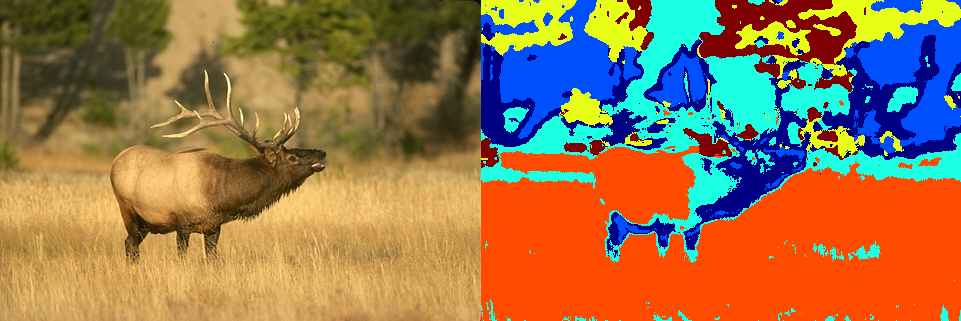
\includegraphics[width=1\linewidth]{41006.png}
\end{center}
   \caption{Ejemplo de segmentación usando kmeans con 6 clusters.}
\label{fig:long}
\label{fig:onecol}
\end{figure}

Se usó el método gmm con diferentes números de clusters. (ver Figura 2.)

\begin{figure*}
\begin{center}
%\fbox{\rule{0pt}{2in} \rule{.9\linewidth}{0pt}}
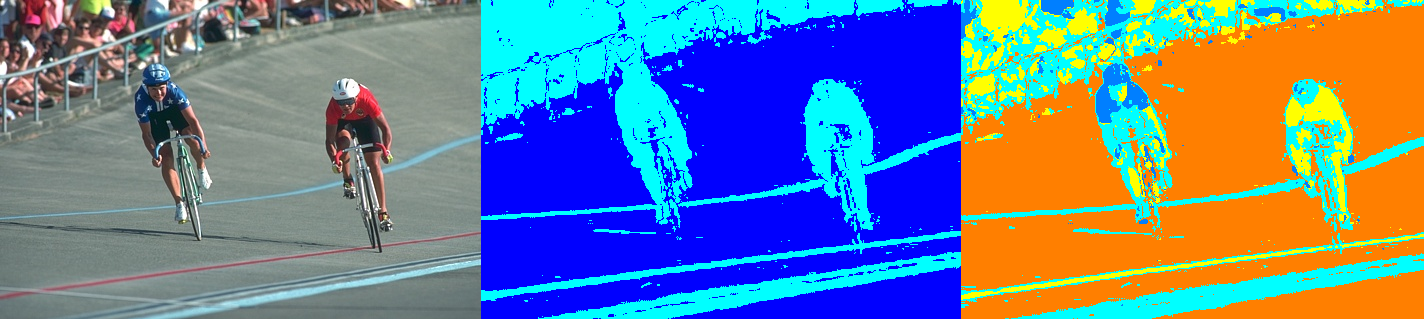
\includegraphics[width=7in]{kmeans_full.png}
\end{center}
   \caption{Ejemplo de una imagen segmentada a partir del método gmm. (Izquierda) imagen original, (centro) imagen segmentada por gmm con k=2 y (derecha) imagen segmentada por gmm con k=4}
\label{fig:short}
\end{figure*}

Watersheds es un método diferente a kmeans y gmm en cuanto a la selección a priori del número de clusters. En este método se controla el umbral al cual se quiere observar el resultado de la segmentación de la imagen (ver Figura 3. )\

Por último el método de segmentación jerárquica crea grupos de clustering de datos a través de una variedad de escalas mediante la creación de un grupo de árboles o dendrograma. El árbol no es un único conjunto de clusters, sino más bien una jerarquía de niveles múltiples, donde los grupos en un nivel se unen como grupos en el siguiente nivel. Esto le permite decidir el nivel o escala de agrupación que es el más apropiado para su aplicación. (ver Figura 4.).

\begin{figure}[t]
\begin{center}

   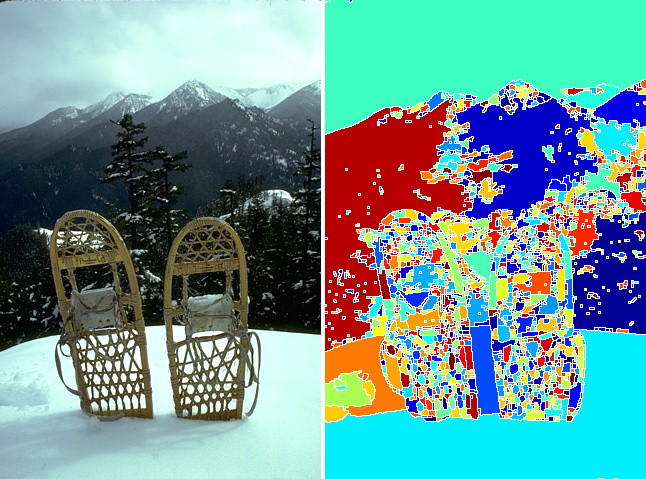
\includegraphics[width=1\linewidth]{Watersheds_ful.png}
\end{center}
   \caption{Ejemplo de segmentación usando Watersheds con un umbral de 10.}
\label{fig:long}
\label{fig:onecol}
\end{figure}

\begin{figure}[t]
\begin{center}
   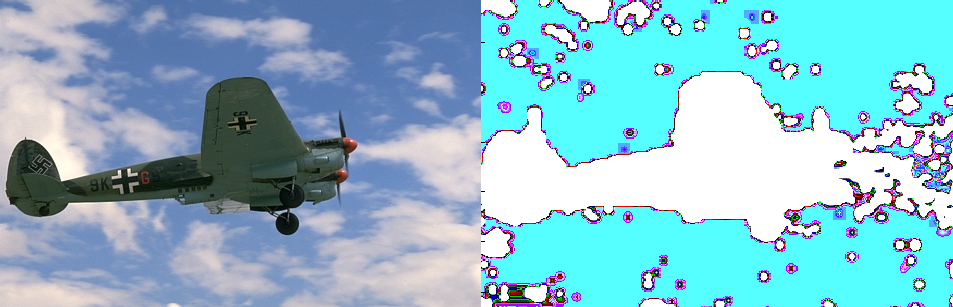
\includegraphics[width=1\linewidth]{3063_l.png}
\end{center}
   \caption{Ejemplo de segmentación jerárquica con un umbral de 10.}
\label{fig:long}
\label{fig:onecol}
\end{figure}

\subsection{Segmentación Imágenes Test de BSDS500}

En total se obtuvieron 800 diferentes segmentaciones, 200 archivos .mat y en cada uno 4 celdas con 4 diferentes segmentaciones por imagen. Estos archivos se guardaron en la carpeta Evaluación\_FJCS\.zip. 


\subsection{Evaluación de Segmentación}

Los resutlados de la evaluación estan dados por tres variables: el valor F para Optima data scale (ODS), el valor F para optimal image scale (OIS) y el área bajo la curva precisión-cobertura. (ver Tabla 1., 2. y 3.).

ODS, usa un umbral fijo para todas las imágenes en el conjunto de datos de evaluación, calibradas para proporcionar un rendimiento óptimo en el conjunto de entrenamiento.

Por el contrario, OIS, evalua el rendimiento de los métodos cuando el umbral (threshold) óptimo es seleccionado por otro algoritmo en función de cada imagen. Con este uno debería obtener mejores segmentaciones.[1]

\begin{table}
\begin{center}
\begin{tabular}{|l|c|}
\hline
Método & Valor ODS \\
\hline\hline
kmeans & F( 0.68, 0.38 ) = 0.49\\
gmm & F(0.71, 0.41) = 0.52  \\
UCM & F( 0.73, 0.73 ) = 0.73\\
\hline
\end{tabular}
\end{center}
\caption{Resultados de F para ODS}
\end{table}

\begin{table}
\begin{center}
\begin{tabular}{|l|c|}
\hline
Método & Valor OIS \\
\hline\hline
kmeans & F( 0.75, 0.44 ) = 0.55\\
gmm & F( 0.74, 0.46 ) = 0.57  \\
UCM & F( 0.77, 0.75 ) = 0.76\\
\hline
\end{tabular}
\end{center}
\caption{Resultados de F para OIS}
\end{table}

\begin{table}
\begin{center}
\begin{tabular}{|l|c|}
\hline
Método & Área \\
\hline\hline
kmeans & 0.15\\
gmm & 0.16  \\
UCM & 0.73\\
\hline
\end{tabular}
\end{center}
\caption{Resultados deL área bajo la curva precisión-cobertura}
\end{table}

\begin{figure}[h]
\begin{center}

   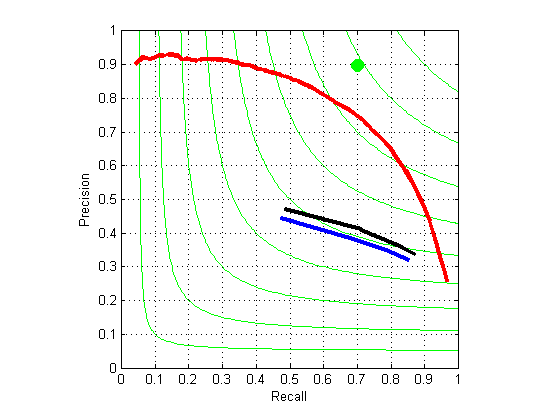
\includegraphics[width=1\linewidth]{isoF_Completa.png}
\end{center}
   \caption{Esta gráfica compara el rendimiento de los métodos kmeans (línea azul) y gmm (línea negra) comparados con el método de UCM (línea roja) de P. Arbeláez[1]}
\label{fig:long}
\label{fig:onecol}
\end{figure}

\section{Discusión y Conclusiones}

Es evidente la inferioridad en rendmiento de lo métodos kmeans y gmm respecto al método propuesto por Arbeláez [1]. Pero es gracias al método de evaluación de curvas que se puede cuantificar las diferencias en estos tres métodos.

Debido a la poca disponibilidad de equipos con alto poder computacional solo se pudieron correr 4 diferentes segmentaciones por imagen (2 a 5 clusters). Esto hace que la curva precisión-cobertura sea muy corta. Es por ello que los valores de área bajo la curva (ver Tabla 3.) no son confiables para comparar los métodos. Sin embargo, el valor F, tanto para ODS como OIS es comparable. Kmeans tiene un valor F menor que gmm aunque no es muy significativo. 

En cuanto a la precisión, la cual es la fracción de instancias recuperadas que son relevantes (verdaderas positivas), el método de kmeans es menor a gmm y ambos son muy inferiores respecto a UCM  y a la misma segmentación por humanos. En cambio, en cobertura, kmeans y gmm tienen valores similares a los humanos,74\% y 75\% respectivamente. Esto quiere decir, que las segmentaciones de kmeans y gmm segmentan con gran porcentaje las segmentaciones que hacen los humanos, pero carecen de precisión. 

Ambos métodos tiene resultados similares y se podrían mejorar usando mayor numeros de clusters en su evaluación. Al ser kmeans y gmm, un tipo de segmentación no supervisada, se podría mejorar añadiendo algún tipo de segmentación supervisada.

\section{Referencias}

\begin{quote}

   [1] P. Arbelaez, M. Maire, C. Fowlkes and J. Malik. ''Contour Detection and Hierarchical Image Segmentation''. IEEE TPAMI, Vol. 33, No. 5, pp. 898-916, May 2011..
\end{quote}

{\small
\bibliographystyle{ieee}
\bibliography{egbib}
}

\end{document}
